\section{Triplon Excitations in the VBS}\label{sec:triplon_bond_operator}

Having found an exact mapping between the VBS phases we now focus on the singlet VBS  around $\varphi = \pi$. Our objective is to find an effective description of this phase and analyse its excitation spectrum. The numerics indicate that spin singlets form on the inter-triangle bonds, thus we shall start by pairing the spins on these bonds and transform to the bond operator representation introduced by Sachdev and Bhatt~\cite{sachdev_bond-operator_1990, gopalan_spin_1994}. Spins on a given bond are labelled with $\sigma_L$ and $\sigma_R$, and treated as a single site, collapsing the star lattice into a Kagome lattice, as shown in Fig.~\ref{fig:lattice_to_kagome}. We can then rewrite the Hamiltonian in a two-spin basis for each dimerised bond, given by Eqns.~\ref{eqn:s_def}-\ref{eqn:tz_def}.
\begin{figure}[t]
    \centering
    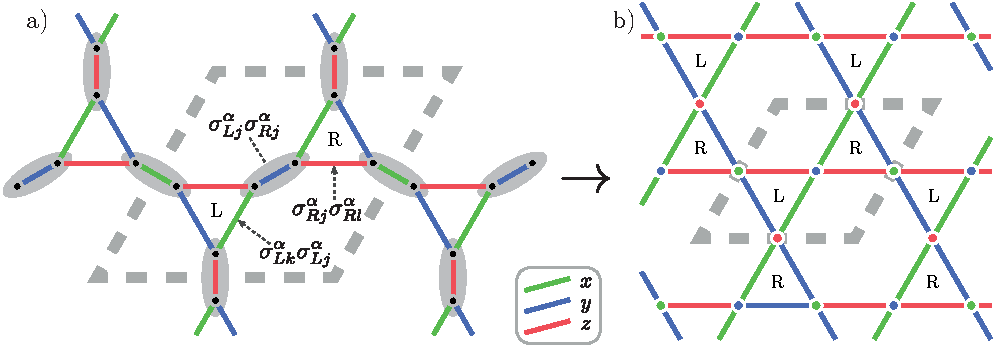
\includegraphics[]{kitaev_heisenberg_star/figures/triplon_latttice.pdf}
    \caption{ 
    \textbf{(a)}~Diagram of the lattice with positions of spin singlets highlighted in grey. Spins are labelled as $\sigma_{R/L}$ depending on which triangle they form a part of in the unit cell. \textbf{(b)}~The derived Kagome lattice once all the singlets are collapsed to a single site. Here, both edges and sites have a Kitaev labelling $\alpha \in {x,y,z}$, denoted by colour. }
    \label{fig:lattice_to_kagome}
\end{figure}

In order to apply mean field theory, let us re-express these states in terms of bosonic creation operators. Starting with a vacuum $\ket 0$ which contains no particles whatsoever, we define four bosonic creation operators that create singlet and triplet states,
$ s^\dag \ket 0 = \ket s$, 
$ t_\alpha^\dag \ket 0 = \ket {t_\alpha}$, which satisfy the relevant commutation relations,
$[s, s^\dag] = 1$, 
$[t_\alpha, t_\beta^\dag] = \delta_{\alpha \beta}$, 
$[s, t_\alpha^\dag] = 0$. In this basis, the spin operators take the following form
\begin{align}
    \sigma_L^\alpha &= -i(s^\dag t_\alpha - t^\dag_\alpha s) - i\varepsilon _{\alpha \beta \gamma} t^\dag_\beta t_\gamma,\\ 
    \sigma_R^\alpha &= i(s^\dag t_\alpha - t^\dag_\alpha s) - i\varepsilon _{\alpha \beta \gamma} t^\dag_\beta t_\gamma.
\end{align}
Of course, in doing so we have artificially enlarged our Hilbert space. For a state to be legitimate, all sites must be populated by a single boson -- any state with empty or multiply occupied sites will be in the `unphysical' part of the extended Hilbert space. Thus, we introduce a chemical potential term to $H$ that enforces single occupancy per site on average,
\begin{align}
    H_\mu = - \sum_{j \in  \mathcal D}
    \mu \left (
     s_j^\dag s_j + t_{\alpha j } ^\dag t_{\alpha j } - 1 
    \right ).
\end{align}
Additionally, we shall model the effect of an applied magnetic field on our triplon bands. For an arbitrary field $\textbf h = (h_x, h_y, h_z)$, the magnetic term in $H$ is 
$H_{h} = -\sum_{j} h_{\alpha}(\sigma^\alpha_{jL} + \sigma^\alpha_{jR})$, which, when expressed in terms of our triplon operators, becomes
\begin{align}
    H_h = \sum_{j}h_\alpha 2i\varepsilon_{\alpha \beta \gamma} t^\dag_\beta t_\gamma.
\end{align}
Since we expect the system to form a singlet VBS, let us introduce a real singlet condensate density order parameter $\bar s = \braket{s_j}$. The three dimers in the unit cell (shown in Fig.~\ref{fig:lattice_to_kagome}a) are equivalent by $C_3$ rotation, so we may describe all singlets with the same $\bar s$. Finally, the total Hamiltonian can be rewritten as
\begin{align} \label{eqn:triplon_hamiltonian}
    H &=H_0 + H_2 + H_4,
\end{align}
with
\begin{align}
    H_0 &=  N\left [ \bar s^2 (K + 2 J - \mu)  + \mu\right ],
\\
    \begin{split}
    H_2 &=  \sum_{j \in  \mathcal D} 
    (K - 2 J - \mu) t_{\alpha j}^\dag t_{\alpha j} 
    - (K+\mu) t_{\bar \alpha j }^\dag t_{\bar \alpha j }
    +h_\alpha 2i\varepsilon_{\alpha \beta \gamma} t^\dag_\beta t_\gamma 
\\
    &\quad - \sum_{jk \in \mathcal D, \alpha} 
    J^\alpha _{jk} \bar s^2 \left (
     t_{\alpha k}^\dag t_{\alpha j} 
    - t_{\alpha j} t_{\alpha k} + h.c.
    \right ),
    \end{split}
\\
    H_4 &=  - \sum_{jk \in \mathcal D, \alpha} J^\alpha _{jk} 
    \left (
    t_{bj}^\dag t_{bk} t_{ck}^\dag t_{cj} 
    - t_{bj}^\dag t_{bk}^\dag t_{cj} t_{ck} + h.c.   
    \right ),
\end{align}
where the parameter $J^\alpha_{jk}$ represents either $K$ or $J$, depending on whether $\alpha$ matches the bond colouring or not. In $H_4$, the indices $b$ and $c$ describe the two directions that do not match $\alpha$. Note that we have discarded terms with three $t_\alpha$\footnote{The Kagome lattice admits a reflection that swaps L and R triangles, which reverses the sign of the triple $t$ terms. Since the original spin system is invariant to this transformation we expect that these terms should vanish.}.

\begin{figure}
    \centering
    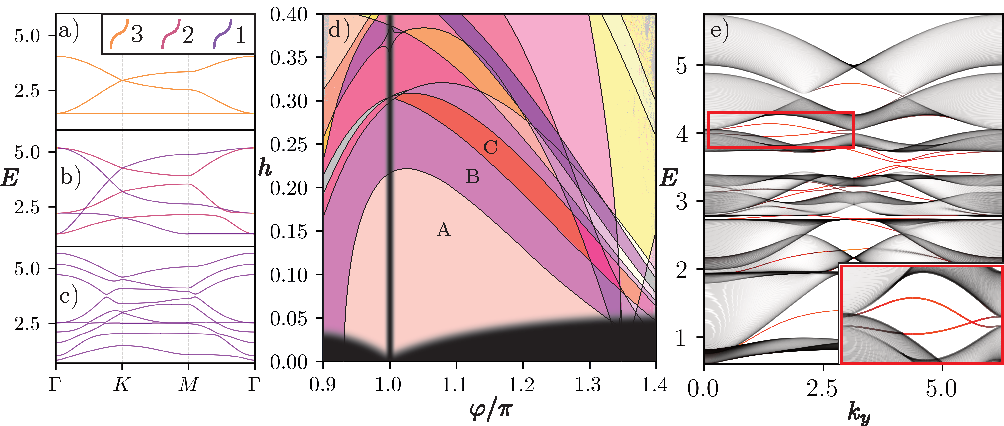
\includegraphics[]{kitaev_heisenberg_star/figures/triplons.pdf}
    \caption {\textbf{(a-c)} Triplon excitation band structure, with the degeneracy of each energy indicated by line colour --  a legend is provided at the top of panel a. 
    \textbf{(a)}~Band structure for the pure Heisenberg case ($\varphi = \pi$) with no applied field. The triple degenerate energy levels correspond to states $t_\alpha$ with $\alpha = x,y,z$. 
    \textbf{(b)}~The band structure for a system with some Kitaev anisotropy ($\alpha = 1.25\pi \implies K \sim -2.1, J\sim -0.71 $) and zero magnetic field. Here the triple degenerate bands are split into one double degenerate band and one non-degenerate band, however all bands remain gapless. 
    \textbf{(c)}~The band structure in the above case ($\varphi = 1.25\pi$), with an applied magnetic field ($h = 0.15$). Here we see that all bands are non-degenerate and gapped. 
    \textbf{(d)}A plot showing the rich phase diagram of possible Chern numbers for the nine triplon bands as a function of the two parameters: Kitaev anisotropy ($\alpha$) and applied magnetic field ($h$). Regions where the bands are gapless are indicated in black and regions where the numerical process failed to converge to a stable solution are shown in grey. Each area with a distinct colouring represents a different set of the Chern numbers of the nine bands. For example the region labelled $A$ has Chern numbers $(-1, 3, -5, 6, -6, 6, -5, 3, -1)$, the $B$ region has $(-1, 3, -5, 6, -6, 3, -2, 3, -1)$, and the $C$ region has $(-1, 3, 1, 0, -6, 3, -2, 3, -1)$.
    \textbf{(e)}~Band structure for a strip system with periodic boundaries in the $y$-direction and open boundaries in the $x$-direction. We have set $\varphi = 1.25\pi$, $h = 0.15$ - thus are in region $B$. Bands are plotted as a function of $k_y$ for a strip containing 130 unit cells in the $x$-direction. States are coloured by their inverse participation ratio, $\textup{IPR} = \sum_{x} |\psi(x)|^4$, where red indicates a localised edge mode, and grey indicates a delocalised bulk mode. Inset shows an enlarged section of the band structure, where a pair of edge modes can be seen connecting two otherwise gapped bands. 
    }
    \label{fig:triplon_results}
\end{figure}

Finally, the quartic terms can be decoupled by introducing the following standard mean-fields
\begin{align} \label{eqn:pqself_consistency}
    P_{jk}^\alpha &= \braket{t_{j\alpha}^\dag t_{k\alpha}} 
    \\ \label{eqn:pqself_consistency2}
    Q _{jk}^\alpha &= \braket{t_{j\alpha} t_{k\alpha}}
\end{align}
Thus, we are left with a quadratic Hamiltonian $H_{MF}(\mu, \bar s, P^\alpha_{jk} , Q^\alpha_{jk} )$ for the triplons  and the four parameters are determined self-consistently. A valid ground state is given by choosing $\mu$ and $\bar s$ such that the Hamiltonian satisfies the saddle point equations
\begin{align} \label{eqn:triplon_saddle_point}
    \left \langle
        \frac
        {\partial H_{MF}}
        {\partial \mu} 
    \right \rangle
    =
    \left \langle
        \frac
        {\partial H_{MF}}
        {\partial \bar s} 
    \right \rangle
    =0,
\end{align}
where the expectation value is calculated in the ground state. Furthermore, $P$ and $Q$ must satisfy the self-consistency relations (Eqns.~\ref{eqn:pqself_consistency} and \ref{eqn:pqself_consistency2}). Self-consistent values for $\mu, \bar s, P$ and $Q$ are determined by using a root finding algorithm (\texttt{scipy.optimize.root}) to converge to a set of mean fields that satisfy these conditions. At each step of the iteration, the Hamiltonian is solved using the bosonic Bogoliubov-de-Gennes method~\cite{blaizot_quantum_1986}, and the mean fields are determined from the bosonic ground state. Details for the method are given in Appendix \ref{apx:triplon_mean_field_theory}.

We now investigate the triplon excitation spectrum obtained from the self-consistently determined Hamiltonian. Since the unit cell contains 3 sites, each hosting three triplon states, the excitation spectrum will contain 9 energy levels. Provided these are gapped, the Chern number of each band can be calculated. A detailed description of the Bogoliubov-de-Gennes method and how the topological invariants are obtained is provided in Appendix~\ref{apx:boson_bdg}.

Triplon spectra were determined using two parameters to tune the Hamiltonian. The Kitaev anisotropy (i.e.~the relative strength of $K/J$) was controlled by sweeping over a range of $\varphi \in [0.9\pi, 1.4\pi]$, approximately the range over which the system forms a stable VBS. Additionally, we applied a magnetic field in the $(1,1,1)$ direction, sweeping over a range of field strengths $h_{\alpha} = h \in [0,0.35]$. The results for these calculations are shown in Fig.~\ref{fig:triplon_results}. 

In the pure Heisenberg limit, we have three exactly degenerate triplon bands, each corresponding to a $t_x$, $t_y$ or $t_z$-type excitation, with a Dirac-like band touching at the $\Gamma$ point. In order to allow for topological excitations to form, two ingredients are needed: gaps need to be opened between the bands, and TRS must be broken to allow for non-zero Chern number. Applying a magnetic field to the Heisenberg system is not sufficient for topological bands, as a field simply splits the three degenerate triplons with an energy shift, producing a $\ket {\uparrow \uparrow}$ state aligned with the field with slightly lower energy, a $\ket {\downarrow \downarrow}$ state with slightly higher energy, and a $\ket{\uparrow \downarrow}+\ket{\downarrow \uparrow}$ band that is unaffected. Similarly, introducing only a Kitaev anisotropy $\varphi \neq \pi$ is also insufficient as the bosonic Hamiltonian retains TRS. Spectra for these cases are shown in Fig.~\ref{fig:triplon_results}a and b.

However, in the presence of both a magnetic field and the Kitaev anisotropy, the system generally has nine distinct gapped triplon bands, shown in Fig.~\ref{fig:triplon_results}c. Most interestingly, the bands have a rich phase diagram of possible Chern numbers depending on these two parameters. A full phase diagram is shown in Fig.~\ref{fig:triplon_results}d. With open boundaries, the bands then have chiral triplon edge modes by the bulk-edge correspondence, an example is shown in Fig.~\ref{fig:triplon_results}e.